\subsection{Infrastructure mise en place}
    Nous avons réalisé un prototype basé sur Docker. Notre objectif était de déployer une version simplifiée de l'architecture proposée dans le sujet du projet. Nous avons donc déployé un broker JMS grâce à ActiveMQ dans un conteneur Docker. Nous avons intégré ce conteneur dans une chaîne d'intégration continue, reposant sur TravisCI et un répertoire Git public hébergé sur GitHub à l'adresse \url{https://github.com/AntoineAugusti/projet-CASI}. Nous nous sommes inspirés de la documentation de TravisCI pour mettre en place cette chaîne d'intégration continue\cite{travisDocker}.\\

    Notre script de déploiement du broker JMS est visible à l'adresse suivante: \url{https://github.com/AntoineAugusti/projet-CASI/blob/master/deployBroker.sh}. Celui-ci utilise un conteneur Docker mis à disposition sur Docker Hub, la plateforme de partage de conteneurs Docker. Ce conteneur comporte ActiveMQ en version 5.12.0 avec OpenJDK-jre-8 sur le système d'exploitation Ubuntu 15.10. Nous avons adapté la configuration à nos besoins. Notre fichier de configuration TravisCI, contenu dans le fichier \texttt{.travis.yml} suivant \url{https://github.com/AntoineAugusti/projet-CASI/blob/master/.travis.yml} s'occupe de lancer le conteneur du broker JMS et de vérifier que les ports 8161 (console d'administration web d'ActiveMQ) et 61616 (point d'entrée du broker JMS) sont accessibles. C'est ce fichier de configuration qui régit le comportement de la chaîne d'intégration continue.

\subsection{Comportements testés}
    Avec la configuration décrite précédemment, nous pouvons nous assurer que le téléchargement du conteneur depuis Docker Hub est possible, que le lancement du conteneur ne pose pas de problème et que les ports mentionnés précédemment sont bien accessibles. Comme la chaîne d'intégration continue a été configurée, ces tests seront effectués à chaque nouveau commit sur le répertoire Git, qui a été push sur GitHub. Un exemple de build s'étant déroulé avec succès sur TravisCI est présenté dans la figure~\ref{fig:travis-build-success} et est visible à l'adresse suivante \url{https://travis-ci.org/AntoineAugusti/projet-CASI/builds/99801715}.

    \begin{figure}[H]
        \centering
        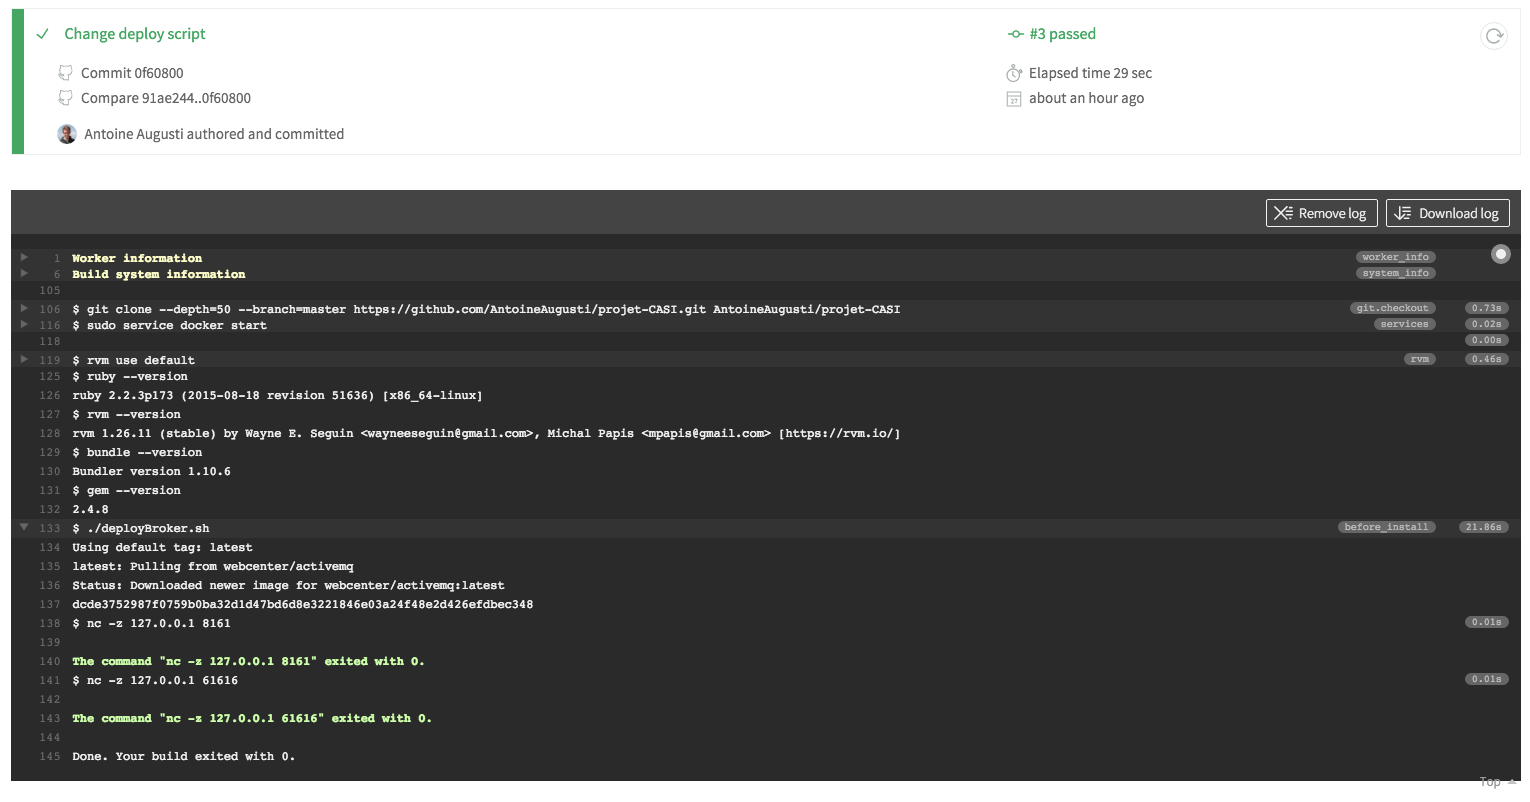
\includegraphics[width=\textwidth]{images/travis-build-success.png}
        \caption{Build s'étant terminé avec succès sur TravisCI}
        \label{fig:travis-build-success}
    \end{figure}

    Pour prouver que notre chaine d'intégration continue fonctionnait, nous avons créé une pull request mappant le port 8161 du conteneur vers le port 8160 de la machine hôte, en omettant de mettre à jour les tests. Le comportement attendu est un échec, puisque le port 8161 ne doit plus être accessible depuis la machine hôte, sur laquelle a été déployée le conteneur. Ceci a été vérifié dans la pull request suivante: \url{https://github.com/AntoineAugusti/projet-CASI/pull/2}. Le build s'étant soldé par un échec sur TravisCI est présenté dans la figure~\ref{fig:travis-build-failure} et est visible à l'adresse suivante \url{https://travis-ci.org/AntoineAugusti/projet-CASI/builds/99801910}.

    \begin{figure}[H]
        \centering
        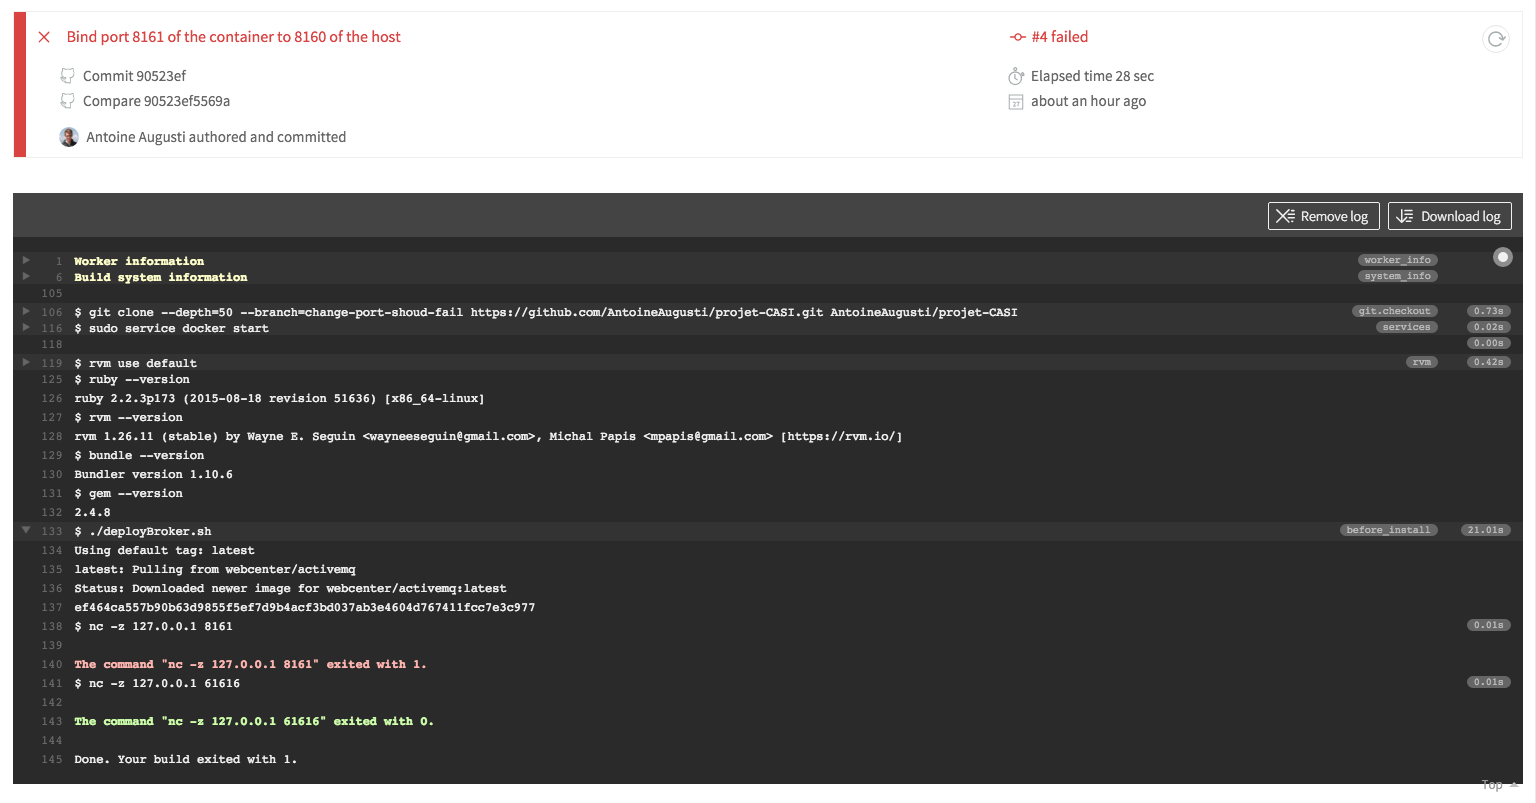
\includegraphics[width=\textwidth]{images/travis-build-failure.png}
        \caption{Build s'étant terminé avec succès sur TravisCI}
        \label{fig:travis-build-failure}
    \end{figure}

    Grâce à ce prototype, nous avons un début de test d'infrastructure, permettant de détecter des anomalies de configuration et pouvant être déployé dans plusieurs environnements (machine d'un développeur, chaine d'intégration continue, serveurs dédiés, plateforme cloud\dots).

\subsection{Métriques mesurées}
    Nos métriques sont basées sur l'installation, le déploiement et l'exécution de tests sur la plateforme de TravisCI.
    \begin{itemize}
        \item Number of failures: 0
        \item Operation time: 29s
        \item CPU: nous n'avons pas réussi à mesurer ceci
        \item Number of installation steps: 2
        \item Number of setup operations: 2
        \item Number of steps / number of setup operations = number of steps by setup operation: 6/2 = 3
        \item Number of test cases: 2
        \item Number of failure + Number of breakdowns x 10: 0
    \end{itemize}
